\documentclass[12pt,a4paper]{report}
\usepackage[utf8]{inputenc}
\usepackage{amsmath}
\usepackage{amsfonts}
\usepackage{amssymb}
\usepackage{graphicx}

\title{Relatório 1  \\
	Projeto em Eletrônica I - EEL7801 \\ \vfill
	\normalsize{Universidade Federal de Santa Catarina - UFSC \\
		Professora: Daniela Ota Hisayasu Suzuki}
	\author{
		{Luiz Augusto Frazatto Fernandes: \it{17202752}} \\
		{Leonardo José Held: \it{17203984}}
	}
}
\date{6 de Junho de 2019}
\begin{document}
	\maketitle
	\setcounter{chapter}{0}
	\chapter{Amplificadores e teste}
	\section{Amplificador - Emissor}
		\paragraph{} Utilizando o CI $LM386$, fez-se um amplificador do sinal sonoro. O circuito fora descrito no Relatóio 1. Uma mudança relevante, no entanto, é em relação ao ganho do circuito: não encontramos um capacitor de que se encaixasse nas especificações sugeridas pelo fabricante ($C = 10\mu{F}$), logo, deixamos o circuito aberto nos pinos de ganho (P8 e P1). O ganho fora limitado a 20 em função dessa alteração.\\
		
		\begin{figure}[h]
			\centering
			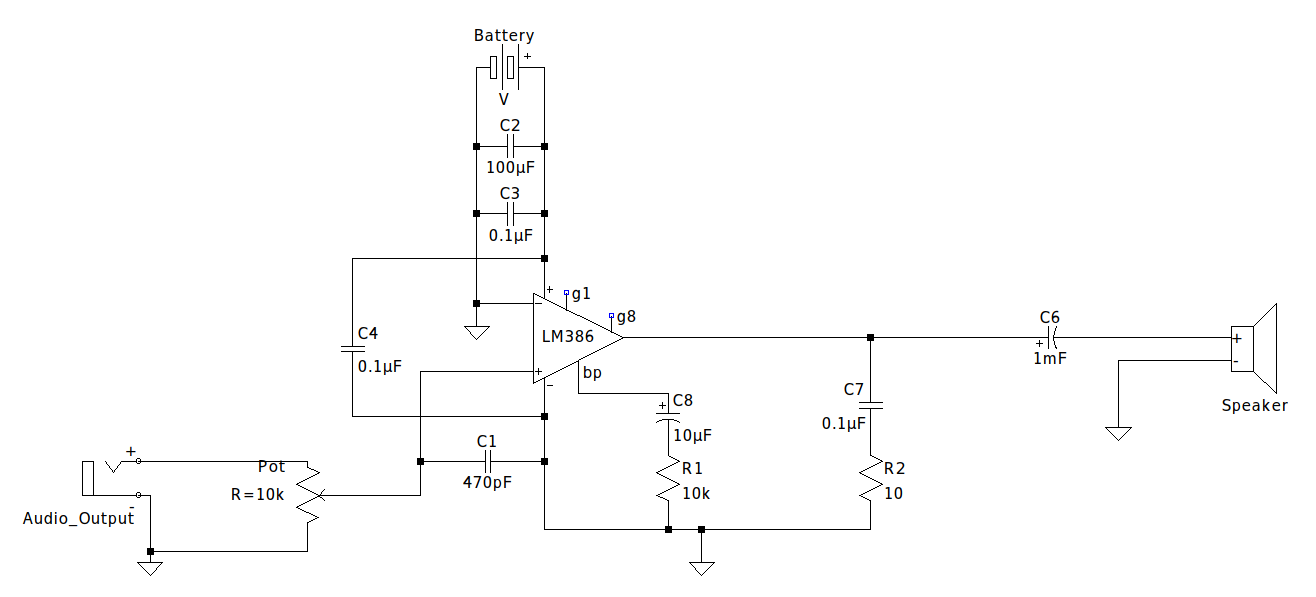
\includegraphics[width=\linewidth]{corrected_amplifier.png}
			\caption{Amplificador com LM386}
			\label{fig:amplifier386}
		\end{figure}
		
		
		\begin{figure}[h]
			\centering
			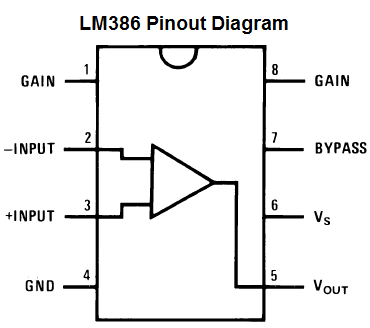
\includegraphics[width=.3\linewidth]{LM386_pinout_diagram.png}
			\caption{Pinagem LM386}
			\label{fig:pinout386}
		\end{figure}
		
		
	\subsection{Ganhos do sinal}
		\paragraph{} Os ganhos obtidos com o circuito amplificador foram os seguintes:\\
		
		%TODO
		\begin{figure}[h]
			\centering
			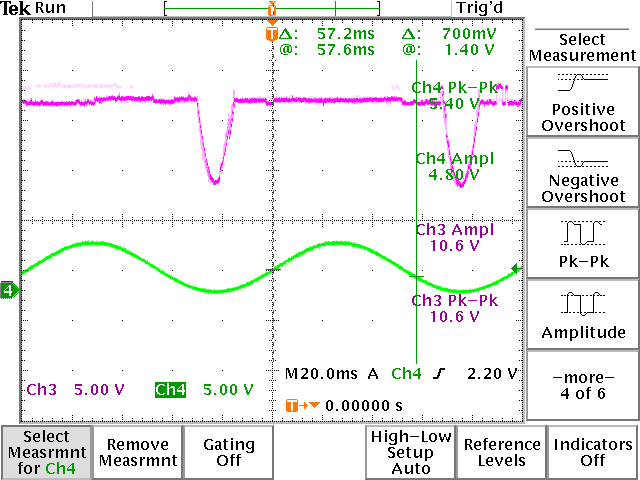
\includegraphics[width=\linewidth]{TEK00003.png}
			\caption{Dados de saída do DAC e do circuito amplificador}
			\label{fig:gainz}
		\end{figure}
	
		Obs.: O sinal original emitido pelo DAC do {\it Bluepill} é representado pelo sinal mais abaixo; o {\it output} gerado pelo {\it OpAmp} é representado pelo sinal cortado. Note que o sinal é saturado pelo {\it OpAmp} ($V_S = 12V$ no $LM386$).
		
		
	\section{Filtro amplificador - Receptor}
		\paragraph{} A fim de se evitar que fossem geradas tensões acima de $5V$ (o Datasheet do MCU recomenda tensões limites de $(5+0.3)V$), colocou-se um diodo zener na saída do circuito, dessa forma limitando o {\it output}. Além disso, caso fosse necessária uma tensão limite de $3.3V$, pode-se colocar um divisor de tensão na saída do regulador. O diodo fora posto após tentativa de se utilizar um regulador de tensão de $5V$, o $LM7805$, mas esse tinha como função, além de limitar a tensão de saída, estabilizá-la, o que prejudicou a análise do sinal (já que esse possui formato de senoide).\\
		
		A resistência mínima a ser colocada em série com o diodo é dado da seguinte maneira:\\
		
		Dados do diodo:
		\begin{itemize}
			\item[1.] Potência: $P_Z = 1W$;
			\item[2.] Tensão: $V_Z = 5.1V$;
		\end{itemize}
		
		Para a obtenção do valor mínimo de resistência que deve ser adicionado em série com o diodo:
		
		\begin{center}
			\begin{gather}
				V_{max} = 12V\\
				V_Z = 5.1V\\
				I_{Zmax} = \frac{V_Z}{P_Z} = 200mA\\
				R_{min} = \frac{V_{max} - V_Z}{I_{max}} = 34.5\Omega\\
			\end{gather}
		\end{center}
		
		Para se garantir a integridade do sinal, mas de ainda termos uma tensão de no máximo $(5 + 0.3)V$, fora colocado na saída do circuito um seguidor de tensão. Esse poderá, no em função de testes futuros a ser retirado do sistema, caso não haja perdas notáveis de potência de sinal se conectado o MCU demodulador ao fim desse primeiro circuito.\\
		
		Houve, além disso, outra mudança importante no circuito: a fim de se evitar que uma corrente insuficiente seja fornecida para o MCU ou a fim de se preservar a integridade do sinal analógico obtido, fez-se um seguidor de tensão, para que esse fosse desacoplado do sinal original. Para tal mudança, optamos pela troca do chip {\it LM741} pelo chip {\it LM324}.
		
		\begin{figure}[h]
			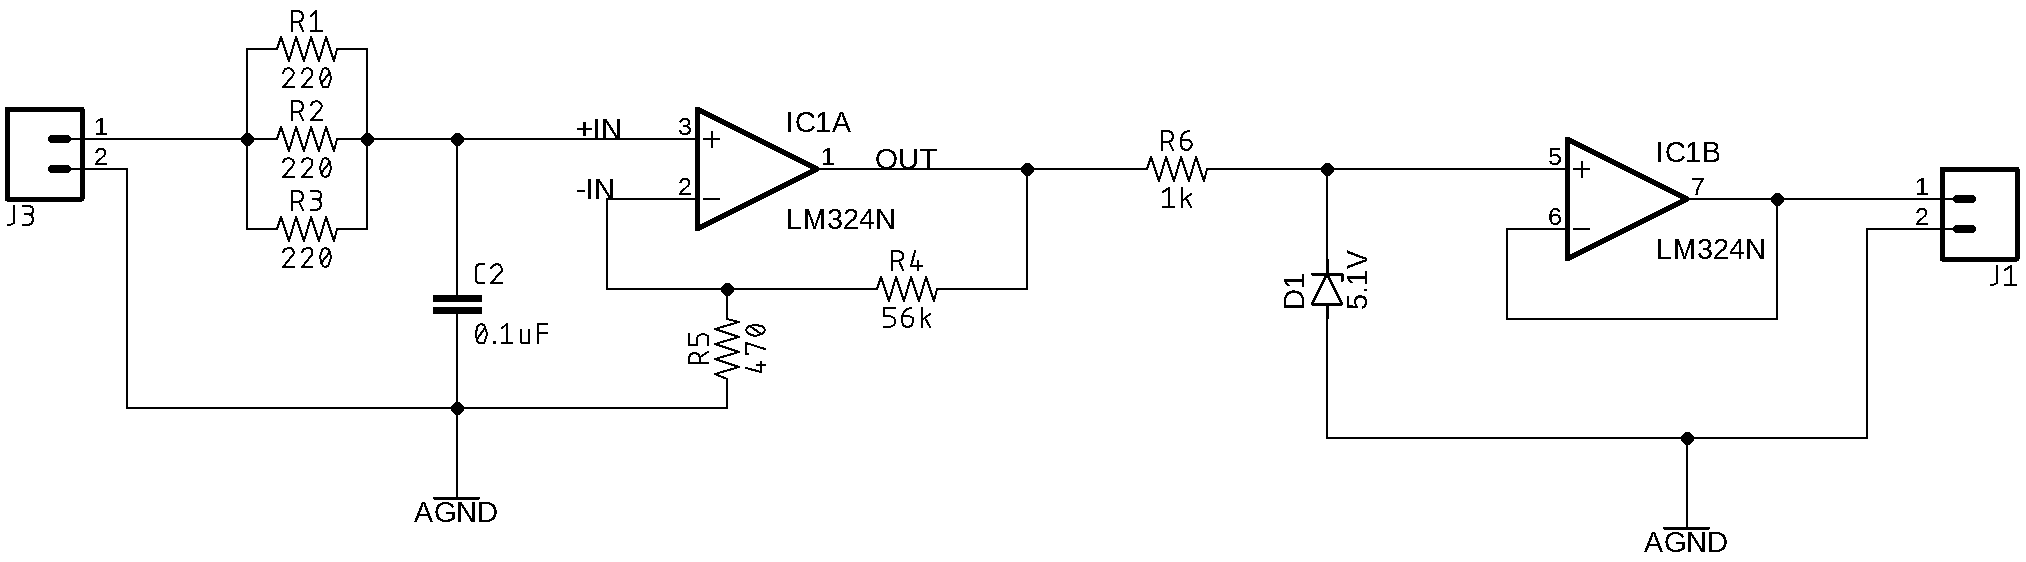
\includegraphics[width=\linewidth]{corrected_filter.png}
			\caption{Filtro passa baixa amplificador. (Obs.: o CI foi alimentado com $V_s = 12V$ e $GND$)}
			\label{fig:filter}
		\end{figure}
			
	\chapter{Implementação Digital}
	
	\section{Módulos D/A e A/D}
	Foi optado por usar dois módulos DCA e ADC externos ao controlador. Ambos usam duas linhas de comunicação I2C pelo mesmo canal.\\
	
	O ADC utilizado foi o {\it ADS1115}, que é um ADC de 16bits (uma resolução que percebemos que seria necessária para o sampling). Ele também conta com um PGA - Programmable Gain Amplifier -, quer permite fazer ajustes de ganho via software.\\
	
	O ADC também possuí 4 canais que enviam para a mesma interface I2C, o que permite uma boa prospecção de expansão do sistema no futuro caso necessário.\\
	
	O DAC utilizado foi o {\it MCP4725}, um DAC de 12 bits, uma resolução bem maior do que o DAC {\it onboard} do Cortex-M3 que estamos usando para controle e computação.\\
	
	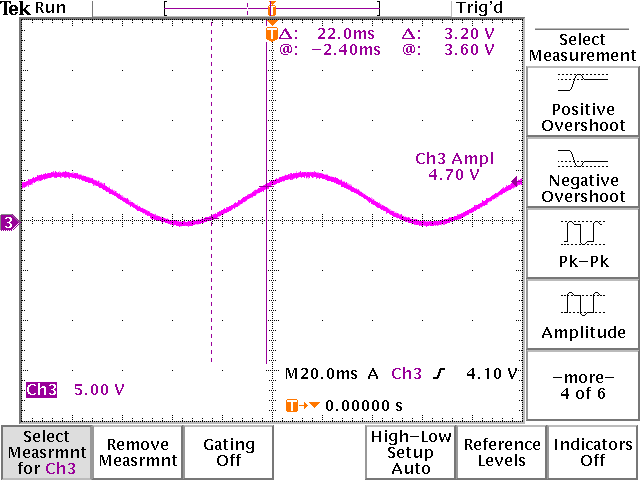
\includegraphics[scale = 0.5]{TEK00000}
	\begin{center}
		\footnotesize{Exemplo de uma Senóide sendo gerada por Lookup Table usando o DAC}
	\end{center}
	\section{Circuito Digital}
	O circuito digital se integra da seguinte maneira com o restante dos amplificadores analógicos:
	
	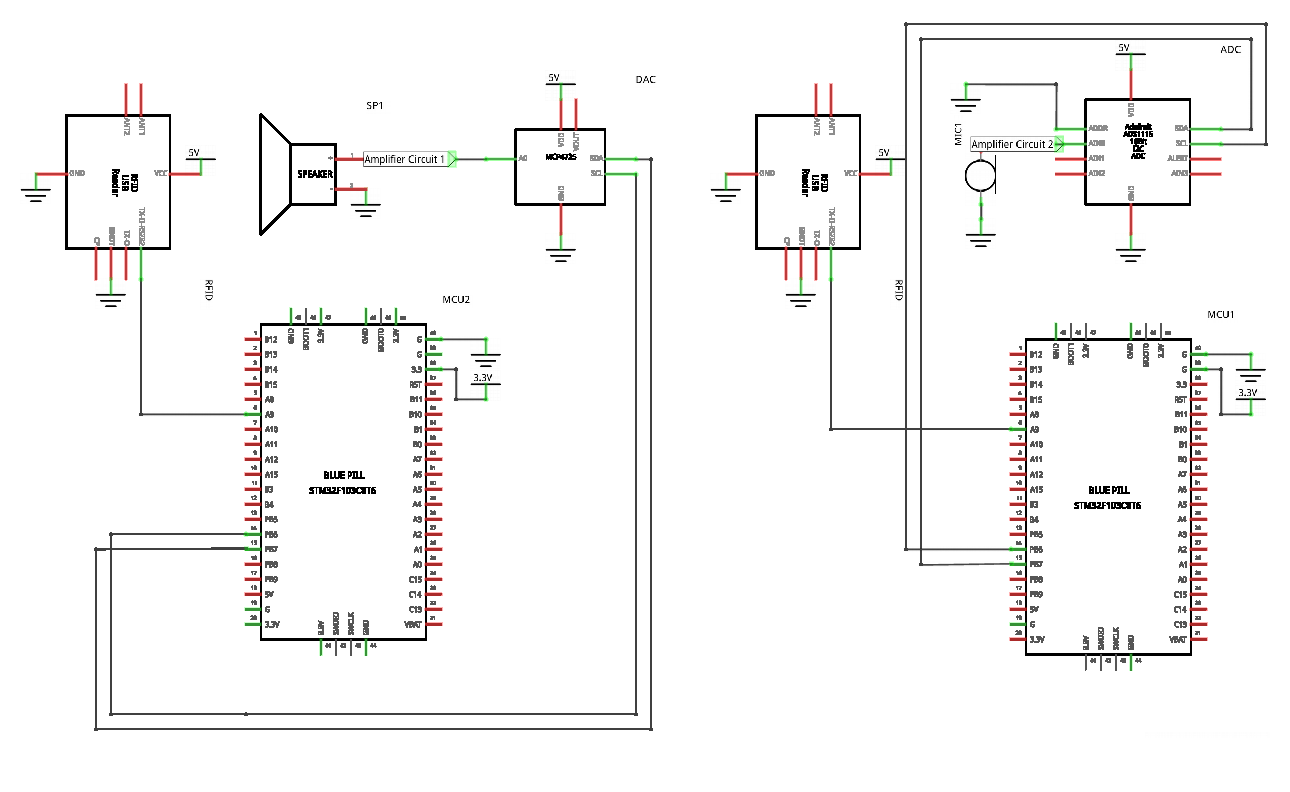
\includegraphics[angle=90,origin=c]{digitaln.pdf}
	
	Basicamente dois Microcontroladores que independentemente controlam uma geração de forma de onda uma aquisição de dados vindos do circuito amplificador do microfone.\\
	
	Como fonte de valores para o D/A, podemos usar o próprio algoritmo gerado em Octave discutido no primeiro relatório. Basta montarmos uma {\it Lookup Table} e passar seus valores para o D/A, gerando uma senóide. 
	
	%todo adicionar Senóide do DA
	
	\chapter{Problemas e Soluções}
	
	\section{Solucionados}
	
	\begin{itemize}
		
		%todo Luiz
		
		\item Comunicação Serial com o Cortex-M3:
		No começo foi utilizado um chip FTDI para fazer a comunicação entre uma das UARTs do Cortex e uma porta serial virtual num computador. O chip FTDI acabou sendo danificado devido um cabo mini-usb faltoso. Para manter os custos baixos, decidimos usar um outro microcontrolador para fazer a conversar $Serial \to USB$. Optamos por usar um mcu que vêm embarcado com quase todas as placas de Arduino, e que realiza a operação.\\
		
		De forma curta: {\it Hackeamos} um embarcado para funcionar como um conversor Serial para os fins de debugging do nosso microcontrolador. No Circuito Digital, estes estão identificados como FTDIs.
		
		\item Resistência em série com o input do DAC:
		
		Nos testes, o ADC estava se comportando de maneira não esperada. O que aconteceu foi que a nossa configuração com o seguidor de linha no final do circuito amplificador desacoplava a corrente, fazendo com que a leitura dos valores não fosse genuína. O problema foi parcialmente resolvido colocando uma resistência em série com a entrada do ADC (inicialmente usamos um potênciometro e decidimos empiricamente o valor utilizado, cerca de 9600 $\Omega$).
		
	\end{itemize}
	
	\section{A serem solucionados}
	
	\begin{itemize}
		\item Transdutor com Intensidade Suficiente:
		O Transdutor que estamos fazendo os testes é um alto-falante extremamente pequeno e limitado em questão de potência. Uma maior intensidade de som parece afetar significativamente a qualidade da conversão Analógica/Digital.
	\end{itemize}
	
	
\end{document}
